\documentclass[1p]{elsarticle_modified}
%\bibliographystyle{elsarticle-num}

%\usepackage[colorlinks]{hyperref}
%\usepackage{abbrmath_seonhwa} %\Abb, \Ascr, \Acal ,\Abf, \Afrak
\usepackage{amsfonts}
\usepackage{amssymb}
\usepackage{amsmath}
\usepackage{amsthm}
\usepackage{scalefnt}
\usepackage{amsbsy}
\usepackage{kotex}
\usepackage{caption}
\usepackage{subfig}
\usepackage{color}
\usepackage{graphicx}
\usepackage{xcolor} %% white, black, red, green, blue, cyan, magenta, yellow
\usepackage{float}
\usepackage{setspace}
\usepackage{hyperref}

\usepackage{tikz}
\usetikzlibrary{arrows}

\usepackage{multirow}
\usepackage{array} % fixed length table
\usepackage{hhline}

%%%%%%%%%%%%%%%%%%%%%
\makeatletter
\renewcommand*\env@matrix[1][\arraystretch]{%
	\edef\arraystretch{#1}%
	\hskip -\arraycolsep
	\let\@ifnextchar\new@ifnextchar
	\array{*\c@MaxMatrixCols c}}
\makeatother %https://tex.stackexchange.com/questions/14071/how-can-i-increase-the-line-spacing-in-a-matrix
%%%%%%%%%%%%%%%

\usepackage[normalem]{ulem}

\newcommand{\msout}[1]{\ifmmode\text{\sout{\ensuremath{#1}}}\else\sout{#1}\fi}
%SOURCE: \msout is \stkout macro in https://tex.stackexchange.com/questions/20609/strikeout-in-math-mode

\newcommand{\cancel}[1]{
	\ifmmode
	{\color{red}\msout{#1}}
	\else
	{\color{red}\sout{#1}}
	\fi
}

\newcommand{\add}[1]{
	{\color{blue}\uwave{#1}}
}

\newcommand{\replace}[2]{
	\ifmmode
	{\color{red}\msout{#1}}{\color{blue}\uwave{#2}}
	\else
	{\color{red}\sout{#1}}{\color{blue}\uwave{#2}}
	\fi
}

\newcommand{\Sol}{\mathcal{S}} %segment
\newcommand{\D}{D} %diagram
\newcommand{\A}{\mathcal{A}} %arc


%%%%%%%%%%%%%%%%%%%%%%%%%%%%%5 test

\def\sl{\operatorname{\textup{SL}}(2,\Cbb)}
\def\psl{\operatorname{\textup{PSL}}(2,\Cbb)}
\def\quan{\mkern 1mu \triangleright \mkern 1mu}

\theoremstyle{definition}
\newtheorem{thm}{Theorem}[section]
\newtheorem{prop}[thm]{Proposition}
\newtheorem{lem}[thm]{Lemma}
\newtheorem{ques}[thm]{Question}
\newtheorem{cor}[thm]{Corollary}
\newtheorem{defn}[thm]{Definition}
\newtheorem{exam}[thm]{Example}
\newtheorem{rmk}[thm]{Remark}
\newtheorem{alg}[thm]{Algorithm}

\newcommand{\I}{\sqrt{-1}}
\begin{document}

%\begin{frontmatter}
%
%\title{Boundary parabolic representations of knots up to 8 crossings}
%
%%% Group authors per affiliation:
%\author{Yunhi Cho} 
%\address{Department of Mathematics, University of Seoul, Seoul, Korea}
%\ead{yhcho@uos.ac.kr}
%
%
%\author{Seonhwa Kim} %\fnref{s_kim}}
%\address{Center for Geometry and Physics, Institute for Basic Science, Pohang, 37673, Korea}
%\ead{ryeona17@ibs.re.kr}
%
%\author{Hyuk Kim}
%\address{Department of Mathematical Sciences, Seoul National University, Seoul 08826, Korea}
%\ead{hyukkim@snu.ac.kr}
%
%\author{Seokbeom Yoon}
%\address{Department of Mathematical Sciences, Seoul National University, Seoul, 08826,  Korea}
%\ead{sbyoon15@snu.ac.kr}
%
%\begin{abstract}
%We find all boundary parabolic representation of knots up to 8 crossings.
%
%\end{abstract}
%\begin{keyword}
%    \MSC[2010] 57M25 
%\end{keyword}
%
%\end{frontmatter}

%\linenumbers
%\tableofcontents
%
\newcommand\colored[1]{\textcolor{white}{\rule[-0.35ex]{0.8em}{1.4ex}}\kern-0.8em\color{red} #1}%
%\newcommand\colored[1]{\textcolor{white}{ #1}\kern-2.17ex	\textcolor{white}{ #1}\kern-1.81ex	\textcolor{white}{ #1}\kern-2.15ex\color{red}#1	}

{\Large $\underline{12a_{0176}~(K12a_{0176})}$}

\setlength{\tabcolsep}{10pt}
\renewcommand{\arraystretch}{1.6}
\vspace{1cm}\begin{tabular}{m{100pt}>{\centering\arraybackslash}m{274pt}}
\multirow{5}{120pt}{
	\centering
	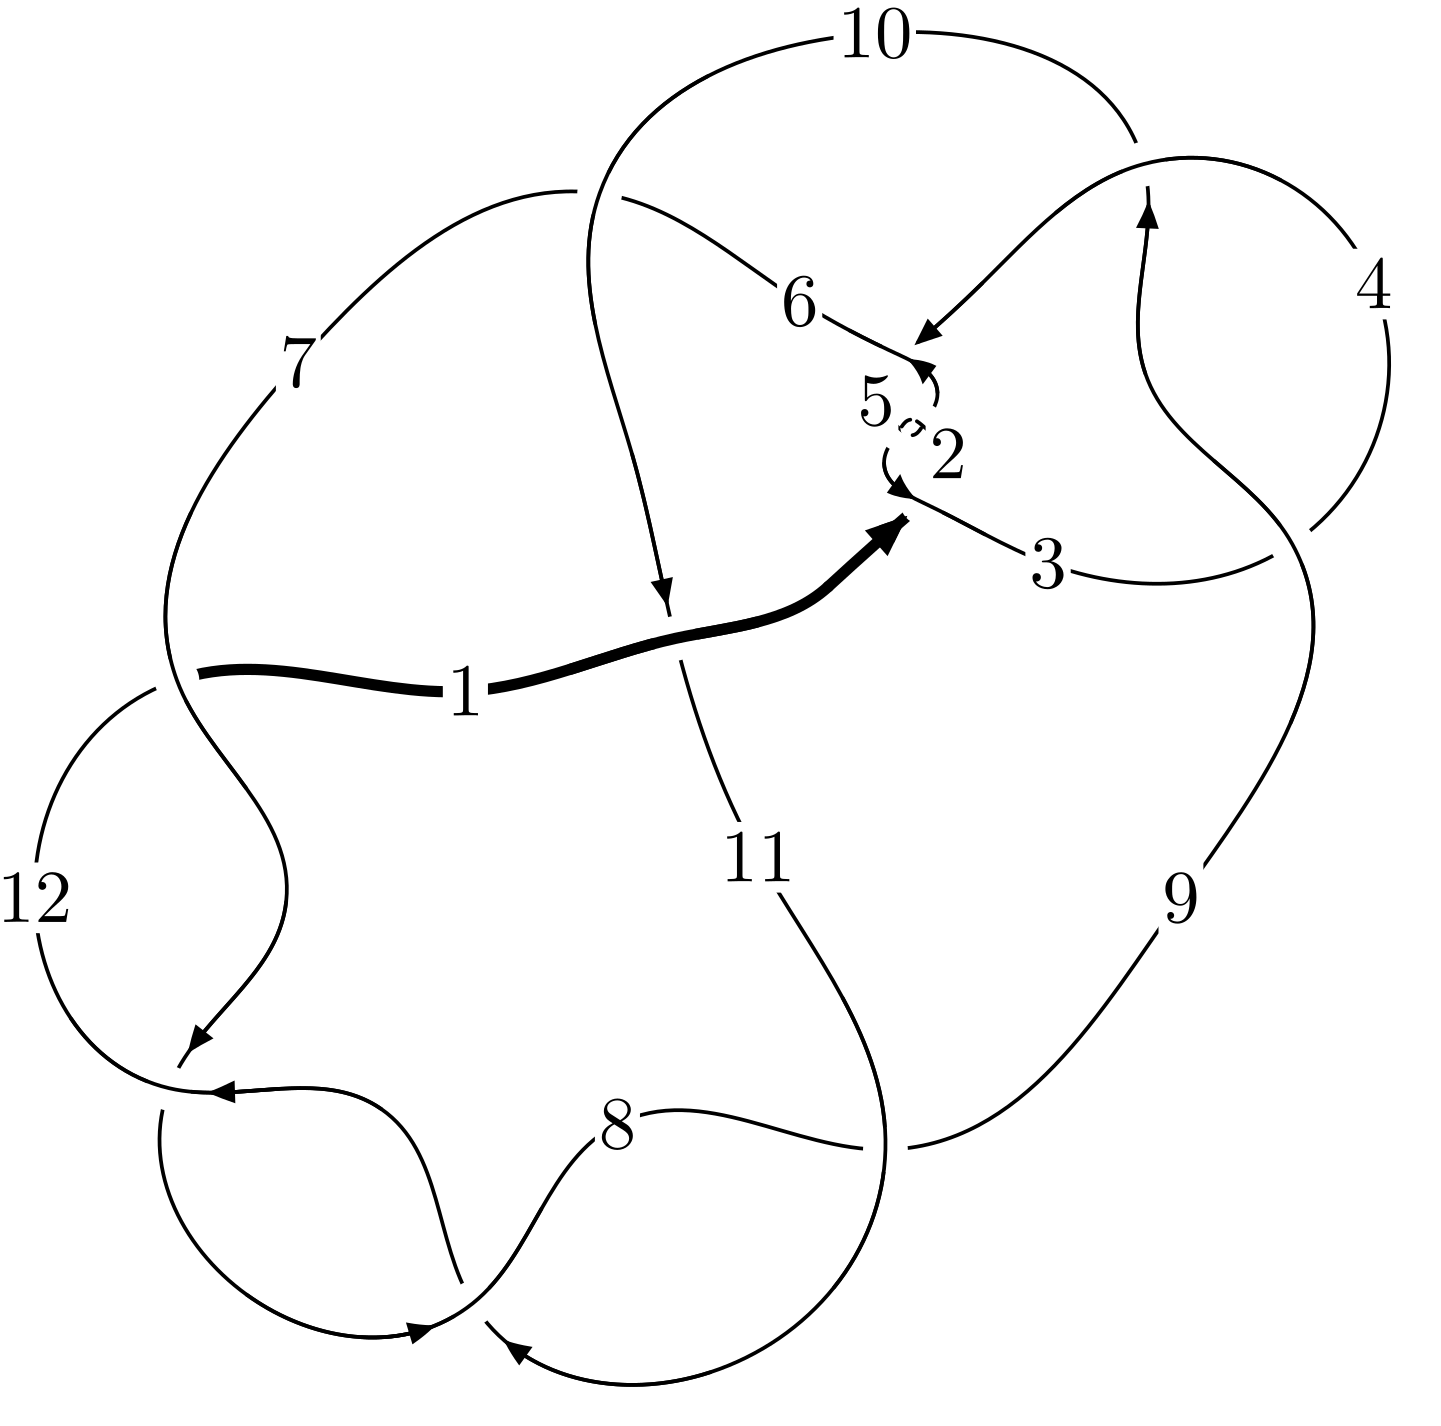
\includegraphics[width=112pt]{../../../GIT/diagram.site/Diagrams/png/977_12a_0176.png}\\
\ \ \ A knot diagram\footnotemark}&
\allowdisplaybreaks
\textbf{Linearized knot diagam} \\
\cline{2-2}
 &
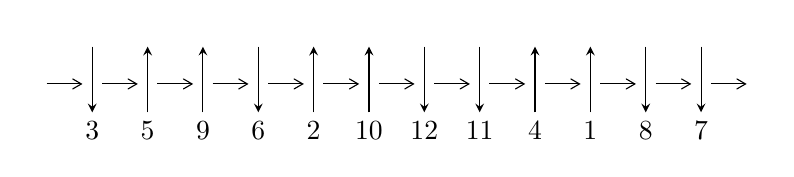
\begin{tikzpicture}[x=20pt, y=17pt]
	% nodes
	\node (C0) at (0, 0) {};
	\node (C1) at (1, 0) {};
	\node (C1U) at (1, +1) {};
	\node (C1D) at (1, -1) {3};

	\node (C2) at (2, 0) {};
	\node (C2U) at (2, +1) {};
	\node (C2D) at (2, -1) {5};

	\node (C3) at (3, 0) {};
	\node (C3U) at (3, +1) {};
	\node (C3D) at (3, -1) {9};

	\node (C4) at (4, 0) {};
	\node (C4U) at (4, +1) {};
	\node (C4D) at (4, -1) {6};

	\node (C5) at (5, 0) {};
	\node (C5U) at (5, +1) {};
	\node (C5D) at (5, -1) {2};

	\node (C6) at (6, 0) {};
	\node (C6U) at (6, +1) {};
	\node (C6D) at (6, -1) {10};

	\node (C7) at (7, 0) {};
	\node (C7U) at (7, +1) {};
	\node (C7D) at (7, -1) {12};

	\node (C8) at (8, 0) {};
	\node (C8U) at (8, +1) {};
	\node (C8D) at (8, -1) {11};

	\node (C9) at (9, 0) {};
	\node (C9U) at (9, +1) {};
	\node (C9D) at (9, -1) {4};

	\node (C10) at (10, 0) {};
	\node (C10U) at (10, +1) {};
	\node (C10D) at (10, -1) {1};

	\node (C11) at (11, 0) {};
	\node (C11U) at (11, +1) {};
	\node (C11D) at (11, -1) {8};

	\node (C12) at (12, 0) {};
	\node (C12U) at (12, +1) {};
	\node (C12D) at (12, -1) {7};
	\node (C13) at (13, 0) {};

	% arrows
	\draw[->,>={angle 60}]
	(C0) edge (C1) (C1) edge (C2) (C2) edge (C3) (C3) edge (C4) (C4) edge (C5) (C5) edge (C6) (C6) edge (C7) (C7) edge (C8) (C8) edge (C9) (C9) edge (C10) (C10) edge (C11) (C11) edge (C12) (C12) edge (C13) ;	\draw[->,>=stealth]
	(C1U) edge (C1D) (C2D) edge (C2U) (C3D) edge (C3U) (C4U) edge (C4D) (C5D) edge (C5U) (C6D) edge (C6U) (C7U) edge (C7D) (C8U) edge (C8D) (C9D) edge (C9U) (C10D) edge (C10U) (C11U) edge (C11D) (C12U) edge (C12D) ;
	\end{tikzpicture} \\
\hhline{~~} \\& 
\textbf{Solving Sequence} \\ \cline{2-2} 
 &
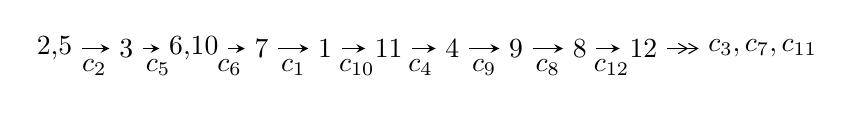
\begin{tikzpicture}[x=23pt, y=7pt]
	% node
	\node (A0) at (-1/8, 0) {2,5};
	\node (A1) at (1, 0) {3};
	\node (A2) at (33/16, 0) {6,10};
	\node (A3) at (25/8, 0) {7};
	\node (A4) at (33/8, 0) {1};
	\node (A5) at (41/8, 0) {11};
	\node (A6) at (49/8, 0) {4};
	\node (A7) at (57/8, 0) {9};
	\node (A8) at (65/8, 0) {8};
	\node (A9) at (73/8, 0) {12};
	\node (C1) at (1/2, -1) {$c_{2}$};
	\node (C2) at (3/2, -1) {$c_{5}$};
	\node (C3) at (21/8, -1) {$c_{6}$};
	\node (C4) at (29/8, -1) {$c_{1}$};
	\node (C5) at (37/8, -1) {$c_{10}$};
	\node (C6) at (45/8, -1) {$c_{4}$};
	\node (C7) at (53/8, -1) {$c_{9}$};
	\node (C8) at (61/8, -1) {$c_{8}$};
	\node (C9) at (69/8, -1) {$c_{12}$};
	\node (A10) at (11, 0) {$c_{3},c_{7},c_{11}$};

	% edge
	\draw[->,>=stealth]	
	(A0) edge (A1) (A1) edge (A2) (A2) edge (A3) (A3) edge (A4) (A4) edge (A5) (A5) edge (A6) (A6) edge (A7) (A7) edge (A8) (A8) edge (A9) ;
	\draw[->>,>={angle 60}]	
	(A9) edge (A10);
\end{tikzpicture} \\ 

\end{tabular} \\

\footnotetext{
The image of knot diagram is generated by the software ``\textbf{Draw programme}" developed by Andrew Bartholomew(\url{http://www.layer8.co.uk/maths/draw/index.htm\#Running-draw}), where we modified some parts for our purpose(\url{https://github.com/CATsTAILs/LinksPainter}).
}\phantom \\ \newline 
\centering \textbf{Ideals for irreducible components\footnotemark of $X_{\text{par}}$} 
 
\begin{align*}
I^u_{1}&=\langle 
93 u^{72}-418 u^{71}+\cdots+8 b-68,\;-11 u^{72}+5 u^{71}+\cdots+8 a-35,\;u^{73}-5 u^{72}+\cdots-7 u+1\rangle \\
I^u_{2}&=\langle 
- a u+b- a,\;a^4- a^3 u- a^2 u- a^2+u,\;u^2+u+1\rangle \\
\\
\end{align*}
\raggedright * 2 irreducible components of $\dim_{\mathbb{C}}=0$, with total 81 representations.\\
\footnotetext{All coefficients of polynomials are rational numbers. But the coefficients are sometimes approximated in decimal forms when there is not enough margin.}
\newpage
\renewcommand{\arraystretch}{1}
\centering \section*{I. $I^u_{1}= \langle 93 u^{72}-418 u^{71}+\cdots+8 b-68,\;-11 u^{72}+5 u^{71}+\cdots+8 a-35,\;u^{73}-5 u^{72}+\cdots-7 u+1 \rangle$}
\flushleft \textbf{(i) Arc colorings}\\
\begin{tabular}{m{7pt} m{180pt} m{7pt} m{180pt} }
\flushright $a_{2}=$&$\begin{pmatrix}1\\0\end{pmatrix}$ \\
\flushright $a_{5}=$&$\begin{pmatrix}0\\u\end{pmatrix}$ \\
\flushright $a_{3}=$&$\begin{pmatrix}1\\- u^2\end{pmatrix}$ \\
\flushright $a_{6}=$&$\begin{pmatrix}u\\u\end{pmatrix}$ \\
\flushright $a_{10}=$&$\begin{pmatrix}\frac{11}{8} u^{72}-\frac{5}{8} u^{71}+\cdots-\frac{269}{8} u+\frac{35}{8}\\-11.6250 u^{72}+52.2500 u^{71}+\cdots-60.3750 u+8.50000\end{pmatrix}$ \\
\flushright $a_{7}=$&$\begin{pmatrix}-\frac{1}{8} u^{72}+\frac{1}{2} u^{71}+\cdots-\frac{1}{8} u-1\\-\frac{1}{8} u^{71}+\frac{1}{2} u^{70}+\cdots+\frac{11}{4} u-\frac{1}{8}\end{pmatrix}$ \\
\flushright $a_{1}=$&$\begin{pmatrix}u^2+1\\- u^4\end{pmatrix}$ \\
\flushright $a_{11}=$&$\begin{pmatrix}\frac{11}{2} u^{72}+4 u^{71}+\cdots-\frac{229}{2} u+\frac{37}{2}\\-26.5000 u^{72}+137.875 u^{71}+\cdots-219.250 u+33.6250\end{pmatrix}$ \\
\flushright $a_{4}=$&$\begin{pmatrix}u^3\\u^3+u\end{pmatrix}$ \\
\flushright $a_{9}=$&$\begin{pmatrix}3.37500 u^{72}+8.12500 u^{71}+\cdots-101.625 u+16.1250\\-23.8750 u^{72}+120.500 u^{71}+\cdots-179.625 u+27.2500\end{pmatrix}$ \\
\flushright $a_{8}=$&$\begin{pmatrix}-1.37500 u^{72}+16.1250 u^{71}+\cdots-58.8750 u+8.62500\\-\frac{101}{8} u^{72}+\frac{243}{4} u^{71}+\cdots-\frac{677}{8} u+13\end{pmatrix}$ \\
\flushright $a_{12}=$&$\begin{pmatrix}\frac{7}{4} u^{72}-\frac{37}{4} u^{71}+\cdots+\frac{37}{2} u-\frac{3}{2}\\\frac{21}{8} u^{72}-\frac{89}{8} u^{71}+\cdots+\frac{63}{8} u-\frac{7}{8}\end{pmatrix}$\\&\end{tabular}
\flushleft \textbf{(ii) Obstruction class $= -1$}\\~\\
\flushleft \textbf{(iii) Cusp Shapes $= -\frac{139}{8} u^{72}+\frac{339}{4} u^{71}+\cdots-\frac{861}{8} u+\frac{73}{4}$}\\~\\
\newpage\renewcommand{\arraystretch}{1}
\flushleft \textbf{(iv) u-Polynomials at the component}\newline \\
\begin{tabular}{m{50pt}|m{274pt}}
Crossings & \hspace{64pt}u-Polynomials at each crossing \\
\hline $$\begin{aligned}c_{1},c_{4}\end{aligned}$$&$\begin{aligned}
&u^{73}+23 u^{72}+\cdots-7 u-1
\end{aligned}$\\
\hline $$\begin{aligned}c_{2},c_{5}\end{aligned}$$&$\begin{aligned}
&u^{73}+5 u^{72}+\cdots-7 u-1
\end{aligned}$\\
\hline $$\begin{aligned}c_{3},c_{9}\end{aligned}$$&$\begin{aligned}
&u^{73}+u^{72}+\cdots-384 u-256
\end{aligned}$\\
\hline $$\begin{aligned}c_{6}\end{aligned}$$&$\begin{aligned}
&u^{73}-3 u^{72}+\cdots+1455 u-1009
\end{aligned}$\\
\hline $$\begin{aligned}c_{7},c_{8},c_{11}\\c_{12}\end{aligned}$$&$\begin{aligned}
&u^{73}-3 u^{72}+\cdots+5 u-1
\end{aligned}$\\
\hline $$\begin{aligned}c_{10}\end{aligned}$$&$\begin{aligned}
&u^{73}+21 u^{72}+\cdots+34585 u+3971
\end{aligned}$\\
\hline
\end{tabular}\\~\\
\newpage\renewcommand{\arraystretch}{1}
\flushleft \textbf{(v) Riley Polynomials at the component}\newline \\
\begin{tabular}{m{50pt}|m{274pt}}
Crossings & \hspace{64pt}Riley Polynomials at each crossing \\
\hline $$\begin{aligned}c_{1},c_{4}\end{aligned}$$&$\begin{aligned}
&y^{73}+59 y^{72}+\cdots-779 y-1
\end{aligned}$\\
\hline $$\begin{aligned}c_{2},c_{5}\end{aligned}$$&$\begin{aligned}
&y^{73}+23 y^{72}+\cdots-7 y-1
\end{aligned}$\\
\hline $$\begin{aligned}c_{3},c_{9}\end{aligned}$$&$\begin{aligned}
&y^{73}-45 y^{72}+\cdots+638976 y-65536
\end{aligned}$\\
\hline $$\begin{aligned}c_{6}\end{aligned}$$&$\begin{aligned}
&y^{73}-39 y^{72}+\cdots-96349267 y-1018081
\end{aligned}$\\
\hline $$\begin{aligned}c_{7},c_{8},c_{11}\\c_{12}\end{aligned}$$&$\begin{aligned}
&y^{73}+85 y^{72}+\cdots-11 y-1
\end{aligned}$\\
\hline $$\begin{aligned}c_{10}\end{aligned}$$&$\begin{aligned}
&y^{73}-19 y^{72}+\cdots+205103581 y-15768841
\end{aligned}$\\
\hline
\end{tabular}\\~\\
\newpage\flushleft \textbf{(vi) Complex Volumes and Cusp Shapes}
$$\begin{array}{c|c|c}  
\text{Solutions to }I^u_{1}& \I (\text{vol} + \sqrt{-1}CS) & \text{Cusp shape}\\
 \hline 
\begin{aligned}
u &= -0.061031 + 0.988224 I \\
a &= \phantom{-}0.443695 - 0.459047 I \\
b &= -0.724621 - 0.580258 I\end{aligned}
 & \phantom{-}3.27771 - 2.37789 I & \phantom{-0.000000 } 0 \\ \hline\begin{aligned}
u &= -0.061031 - 0.988224 I \\
a &= \phantom{-}0.443695 + 0.459047 I \\
b &= -0.724621 + 0.580258 I\end{aligned}
 & \phantom{-}3.27771 + 2.37789 I & \phantom{-0.000000 } 0 \\ \hline\begin{aligned}
u &= -0.225938 + 1.037910 I \\
a &= \phantom{-}0.166934 - 0.176912 I \\
b &= \phantom{-}0.821680 + 0.445687 I\end{aligned}
 & -1.40695 - 2.98844 I & \phantom{-0.000000 } 0 \\ \hline\begin{aligned}
u &= -0.225938 - 1.037910 I \\
a &= \phantom{-}0.166934 + 0.176912 I \\
b &= \phantom{-}0.821680 - 0.445687 I\end{aligned}
 & -1.40695 + 2.98844 I & \phantom{-0.000000 } 0 \\ \hline\begin{aligned}
u &= -0.518783 + 0.940844 I \\
a &= \phantom{-}0.323471 + 0.705744 I \\
b &= \phantom{-}0.015920 + 0.894645 I\end{aligned}
 & -0.10046 - 2.66980 I & \phantom{-0.000000 } 0 \\ \hline\begin{aligned}
u &= -0.518783 - 0.940844 I \\
a &= \phantom{-}0.323471 - 0.705744 I \\
b &= \phantom{-}0.015920 - 0.894645 I\end{aligned}
 & -0.10046 + 2.66980 I & \phantom{-0.000000 } 0 \\ \hline\begin{aligned}
u &= \phantom{-}0.715152 + 0.803648 I \\
a &= \phantom{-}1.139520 + 0.387119 I \\
b &= \phantom{-}0.640803 - 1.009380 I\end{aligned}
 & \phantom{-}8.18684 - 1.63882 I & \phantom{-0.000000 } 0 \\ \hline\begin{aligned}
u &= \phantom{-}0.715152 - 0.803648 I \\
a &= \phantom{-}1.139520 - 0.387119 I \\
b &= \phantom{-}0.640803 + 1.009380 I\end{aligned}
 & \phantom{-}8.18684 + 1.63882 I & \phantom{-0.000000 } 0 \\ \hline\begin{aligned}
u &= -0.373664 + 1.042010 I \\
a &= -0.819992 - 0.035159 I \\
b &= -0.890346 - 0.754074 I\end{aligned}
 & \phantom{-}1.042010 - 0.690934 I & \phantom{-0.000000 } 0 \\ \hline\begin{aligned}
u &= -0.373664 - 1.042010 I \\
a &= -0.819992 + 0.035159 I \\
b &= -0.890346 + 0.754074 I\end{aligned}
 & \phantom{-}1.042010 + 0.690934 I & \phantom{-0.000000 } 0\\
 \hline 
 \end{array}$$\newpage$$\begin{array}{c|c|c}  
\text{Solutions to }I^u_{1}& \I (\text{vol} + \sqrt{-1}CS) & \text{Cusp shape}\\
 \hline 
\begin{aligned}
u &= \phantom{-}0.717261 + 0.854752 I \\
a &= -0.819762 + 0.064738 I \\
b &= -0.019915 + 1.100780 I\end{aligned}
 & \phantom{-}1.69272 + 0.80380 I & \phantom{-0.000000 } 0 \\ \hline\begin{aligned}
u &= \phantom{-}0.717261 - 0.854752 I \\
a &= -0.819762 - 0.064738 I \\
b &= -0.019915 - 1.100780 I\end{aligned}
 & \phantom{-}1.69272 - 0.80380 I & \phantom{-0.000000 } 0 \\ \hline\begin{aligned}
u &= -0.751631 + 0.827950 I \\
a &= \phantom{-}1.75700 - 1.36118 I \\
b &= \phantom{-}2.26394 - 0.53802 I\end{aligned}
 & \phantom{-}3.44600 + 0.21774 I & \phantom{-0.000000 } 0 \\ \hline\begin{aligned}
u &= -0.751631 - 0.827950 I \\
a &= \phantom{-}1.75700 + 1.36118 I \\
b &= \phantom{-}2.26394 + 0.53802 I\end{aligned}
 & \phantom{-}3.44600 - 0.21774 I & \phantom{-0.000000 } 0 \\ \hline\begin{aligned}
u &= -0.703331 + 0.876144 I \\
a &= -1.12934 + 1.54579 I \\
b &= -1.74415 + 1.00598 I\end{aligned}
 & \phantom{-}1.23434 - 2.69793 I & \phantom{-0.000000 } 0 \\ \hline\begin{aligned}
u &= -0.703331 - 0.876144 I \\
a &= -1.12934 - 1.54579 I \\
b &= -1.74415 - 1.00598 I\end{aligned}
 & \phantom{-}1.23434 + 2.69793 I & \phantom{-0.000000 } 0 \\ \hline\begin{aligned}
u &= -0.231481 + 1.101900 I \\
a &= -0.179153 + 0.561689 I \\
b &= -0.892539 - 0.338296 I\end{aligned}
 & \phantom{-}0.16539 - 6.33155 I & \phantom{-0.000000 } 0 \\ \hline\begin{aligned}
u &= -0.231481 - 1.101900 I \\
a &= -0.179153 - 0.561689 I \\
b &= -0.892539 + 0.338296 I\end{aligned}
 & \phantom{-}0.16539 + 6.33155 I & \phantom{-0.000000 } 0 \\ \hline\begin{aligned}
u &= \phantom{-}0.854843 + 0.737463 I \\
a &= -0.97759 - 1.56121 I \\
b &= -1.53845 - 0.36332 I\end{aligned}
 & \phantom{-}5.77476 - 2.35899 I & \phantom{-0.000000 } 0 \\ \hline\begin{aligned}
u &= \phantom{-}0.854843 - 0.737463 I \\
a &= -0.97759 + 1.56121 I \\
b &= -1.53845 + 0.36332 I\end{aligned}
 & \phantom{-}5.77476 + 2.35899 I & \phantom{-0.000000 } 0\\
 \hline 
 \end{array}$$\newpage$$\begin{array}{c|c|c}  
\text{Solutions to }I^u_{1}& \I (\text{vol} + \sqrt{-1}CS) & \text{Cusp shape}\\
 \hline 
\begin{aligned}
u &= \phantom{-}0.877139 + 0.718077 I \\
a &= \phantom{-}1.13328 + 1.73513 I \\
b &= \phantom{-}1.86444 + 0.47628 I\end{aligned}
 & \phantom{-}7.65392 - 6.17000 I & \phantom{-0.000000 } 0 \\ \hline\begin{aligned}
u &= \phantom{-}0.877139 - 0.718077 I \\
a &= \phantom{-}1.13328 - 1.73513 I \\
b &= \phantom{-}1.86444 - 0.47628 I\end{aligned}
 & \phantom{-}7.65392 + 6.17000 I & \phantom{-0.000000 } 0 \\ \hline\begin{aligned}
u &= -0.011705 + 0.860688 I \\
a &= -0.052223 + 0.967136 I \\
b &= \phantom{-}0.932645 + 0.558548 I\end{aligned}
 & -2.42316 - 0.99351 I & -5.92732 + 3.87741 I \\ \hline\begin{aligned}
u &= -0.011705 - 0.860688 I \\
a &= -0.052223 - 0.967136 I \\
b &= \phantom{-}0.932645 - 0.558548 I\end{aligned}
 & -2.42316 + 0.99351 I & -5.92732 - 3.87741 I \\ \hline\begin{aligned}
u &= -0.789311 + 0.824660 I \\
a &= -2.12466 + 1.44766 I \\
b &= -2.66983 + 0.45270 I\end{aligned}
 & \phantom{-}11.52080 + 2.07129 I & \phantom{-0.000000 } 0 \\ \hline\begin{aligned}
u &= -0.789311 - 0.824660 I \\
a &= -2.12466 - 1.44766 I \\
b &= -2.66983 - 0.45270 I\end{aligned}
 & \phantom{-}11.52080 - 2.07129 I & \phantom{-0.000000 } 0 \\ \hline\begin{aligned}
u &= \phantom{-}0.897183 + 0.709153 I \\
a &= -1.23173 - 1.88439 I \\
b &= -2.09388 - 0.61056 I\end{aligned}
 & \phantom{-}15.7401 - 8.6060 I & \phantom{-0.000000 } 0 \\ \hline\begin{aligned}
u &= \phantom{-}0.897183 - 0.709153 I \\
a &= -1.23173 + 1.88439 I \\
b &= -2.09388 + 0.61056 I\end{aligned}
 & \phantom{-}15.7401 + 8.6060 I & \phantom{-0.000000 } 0 \\ \hline\begin{aligned}
u &= \phantom{-}0.715229 + 0.893228 I \\
a &= \phantom{-}0.536474 - 0.487123 I \\
b &= -0.499667 - 1.216460 I\end{aligned}
 & \phantom{-}1.57244 + 4.67543 I & \phantom{-0.000000 } 0 \\ \hline\begin{aligned}
u &= \phantom{-}0.715229 - 0.893228 I \\
a &= \phantom{-}0.536474 + 0.487123 I \\
b &= -0.499667 + 1.216460 I\end{aligned}
 & \phantom{-}1.57244 - 4.67543 I & \phantom{-0.000000 } 0\\
 \hline 
 \end{array}$$\newpage$$\begin{array}{c|c|c}  
\text{Solutions to }I^u_{1}& \I (\text{vol} + \sqrt{-1}CS) & \text{Cusp shape}\\
 \hline 
\begin{aligned}
u &= \phantom{-}0.858736 + 0.779751 I \\
a &= \phantom{-}0.60446 + 1.54193 I \\
b &= \phantom{-}1.076970 + 0.610092 I\end{aligned}
 & \phantom{-}8.88013 + 0.82331 I & \phantom{-0.000000 } 0 \\ \hline\begin{aligned}
u &= \phantom{-}0.858736 - 0.779751 I \\
a &= \phantom{-}0.60446 - 1.54193 I \\
b &= \phantom{-}1.076970 - 0.610092 I\end{aligned}
 & \phantom{-}8.88013 - 0.82331 I & \phantom{-0.000000 } 0 \\ \hline\begin{aligned}
u &= -0.587723 + 1.000390 I \\
a &= -0.51702 - 1.42783 I \\
b &= \phantom{-}0.17444 - 1.64638 I\end{aligned}
 & \phantom{-}6.38689 - 3.34175 I & \phantom{-0.000000 } 0 \\ \hline\begin{aligned}
u &= -0.587723 - 1.000390 I \\
a &= -0.51702 + 1.42783 I \\
b &= \phantom{-}0.17444 + 1.64638 I\end{aligned}
 & \phantom{-}6.38689 + 3.34175 I & \phantom{-0.000000 } 0 \\ \hline\begin{aligned}
u &= -0.236324 + 1.136820 I \\
a &= \phantom{-}0.216812 - 0.826663 I \\
b &= \phantom{-}0.952968 + 0.243595 I\end{aligned}
 & \phantom{-}8.01784 - 8.50189 I & \phantom{-0.000000 } 0 \\ \hline\begin{aligned}
u &= -0.236324 - 1.136820 I \\
a &= \phantom{-}0.216812 + 0.826663 I \\
b &= \phantom{-}0.952968 - 0.243595 I\end{aligned}
 & \phantom{-}8.01784 + 8.50189 I & \phantom{-0.000000 } 0 \\ \hline\begin{aligned}
u &= -0.642269 + 0.533189 I \\
a &= \phantom{-}1.44113 + 0.31196 I \\
b &= \phantom{-}0.909868 + 0.853465 I\end{aligned}
 & \phantom{-}7.73992 - 1.45409 I & \phantom{-}7.03228 + 2.97950 I \\ \hline\begin{aligned}
u &= -0.642269 - 0.533189 I \\
a &= \phantom{-}1.44113 - 0.31196 I \\
b &= \phantom{-}0.909868 - 0.853465 I\end{aligned}
 & \phantom{-}7.73992 + 1.45409 I & \phantom{-}7.03228 - 2.97950 I \\ \hline\begin{aligned}
u &= -0.386720 + 1.102060 I \\
a &= \phantom{-}1.151370 - 0.153712 I \\
b &= \phantom{-}1.145290 + 0.823796 I\end{aligned}
 & \phantom{-}8.94434 + 0.93346 I & \phantom{-0.000000 } 0 \\ \hline\begin{aligned}
u &= -0.386720 - 1.102060 I \\
a &= \phantom{-}1.151370 + 0.153712 I \\
b &= \phantom{-}1.145290 - 0.823796 I\end{aligned}
 & \phantom{-}8.94434 - 0.93346 I & \phantom{-0.000000 } 0\\
 \hline 
 \end{array}$$\newpage$$\begin{array}{c|c|c}  
\text{Solutions to }I^u_{1}& \I (\text{vol} + \sqrt{-1}CS) & \text{Cusp shape}\\
 \hline 
\begin{aligned}
u &= \phantom{-}0.161589 + 0.815556 I \\
a &= \phantom{-}0.08027 + 1.73701 I \\
b &= \phantom{-}1.38565 + 0.62057 I\end{aligned}
 & \phantom{-}5.75319 + 4.41448 I & \phantom{-}0.071981 - 1.204152 I \\ \hline\begin{aligned}
u &= \phantom{-}0.161589 - 0.815556 I \\
a &= \phantom{-}0.08027 - 1.73701 I \\
b &= \phantom{-}1.38565 - 0.62057 I\end{aligned}
 & \phantom{-}5.75319 - 4.41448 I & \phantom{-}0.071981 + 1.204152 I \\ \hline\begin{aligned}
u &= \phantom{-}0.709045 + 0.936655 I \\
a &= -0.200425 + 1.044420 I \\
b &= \phantom{-}1.10352 + 1.40660 I\end{aligned}
 & \phantom{-}7.77191 + 7.10200 I & \phantom{-0.000000 } 0 \\ \hline\begin{aligned}
u &= \phantom{-}0.709045 - 0.936655 I \\
a &= -0.200425 - 1.044420 I \\
b &= \phantom{-}1.10352 - 1.40660 I\end{aligned}
 & \phantom{-}7.77191 - 7.10200 I & \phantom{-0.000000 } 0 \\ \hline\begin{aligned}
u &= \phantom{-}0.085563 + 0.820766 I \\
a &= -0.030152 - 1.397210 I \\
b &= -1.154110 - 0.576548 I\end{aligned}
 & -1.57706 + 2.30309 I & -2.80955 - 3.48929 I \\ \hline\begin{aligned}
u &= \phantom{-}0.085563 - 0.820766 I \\
a &= -0.030152 + 1.397210 I \\
b &= -1.154110 + 0.576548 I\end{aligned}
 & -1.57706 - 2.30309 I & -2.80955 + 3.48929 I \\ \hline\begin{aligned}
u &= -0.736971 + 0.917281 I \\
a &= \phantom{-}1.16448 - 2.10961 I \\
b &= \phantom{-}2.02664 - 1.52743 I\end{aligned}
 & \phantom{-}3.17218 - 5.86940 I & \phantom{-0.000000 } 0 \\ \hline\begin{aligned}
u &= -0.736971 - 0.917281 I \\
a &= \phantom{-}1.16448 + 2.10961 I \\
b &= \phantom{-}2.02664 + 1.52743 I\end{aligned}
 & \phantom{-}3.17218 + 5.86940 I & \phantom{-0.000000 } 0 \\ \hline\begin{aligned}
u &= -0.810712 + 0.097990 I \\
a &= -0.550183 - 0.371106 I \\
b &= \phantom{-}1.117360 - 0.604474 I\end{aligned}
 & \phantom{-}12.19710 - 5.07416 I & \phantom{-}9.95336 + 3.32776 I \\ \hline\begin{aligned}
u &= -0.810712 - 0.097990 I \\
a &= -0.550183 + 0.371106 I \\
b &= \phantom{-}1.117360 + 0.604474 I\end{aligned}
 & \phantom{-}12.19710 + 5.07416 I & \phantom{-}9.95336 - 3.32776 I\\
 \hline 
 \end{array}$$\newpage$$\begin{array}{c|c|c}  
\text{Solutions to }I^u_{1}& \I (\text{vol} + \sqrt{-1}CS) & \text{Cusp shape}\\
 \hline 
\begin{aligned}
u &= \phantom{-}0.885484 + 0.802555 I \\
a &= -0.31616 - 1.77942 I \\
b &= -0.904553 - 1.071020 I\end{aligned}
 & \phantom{-}17.5514 + 2.3531 I & \phantom{-0.000000 } 0 \\ \hline\begin{aligned}
u &= \phantom{-}0.885484 - 0.802555 I \\
a &= -0.31616 + 1.77942 I \\
b &= -0.904553 + 1.071020 I\end{aligned}
 & \phantom{-}17.5514 - 2.3531 I & \phantom{-0.000000 } 0 \\ \hline\begin{aligned}
u &= -0.440972 + 0.666613 I \\
a &= -0.915006 - 0.235271 I \\
b &= -0.765196 - 0.346372 I\end{aligned}
 & \phantom{-}0.70719 - 1.37392 I & \phantom{-}6.54862 + 4.55339 I \\ \hline\begin{aligned}
u &= -0.440972 - 0.666613 I \\
a &= -0.915006 + 0.235271 I \\
b &= -0.765196 + 0.346372 I\end{aligned}
 & \phantom{-}0.70719 + 1.37392 I & \phantom{-}6.54862 - 4.55339 I \\ \hline\begin{aligned}
u &= -0.760835 + 0.932568 I \\
a &= -1.29393 + 2.43000 I \\
b &= -2.28636 + 1.77924 I\end{aligned}
 & \phantom{-}11.18770 - 7.91039 I & \phantom{-0.000000 } 0 \\ \hline\begin{aligned}
u &= -0.760835 - 0.932568 I \\
a &= -1.29393 - 2.43000 I \\
b &= -2.28636 - 1.77924 I\end{aligned}
 & \phantom{-}11.18770 + 7.91039 I & \phantom{-0.000000 } 0 \\ \hline\begin{aligned}
u &= -0.753565 + 0.082487 I \\
a &= \phantom{-}0.721227 + 0.258241 I \\
b &= -0.834537 + 0.418462 I\end{aligned}
 & \phantom{-}4.10320 - 3.11301 I & \phantom{-}8.46380 + 5.00455 I \\ \hline\begin{aligned}
u &= -0.753565 - 0.082487 I \\
a &= \phantom{-}0.721227 - 0.258241 I \\
b &= -0.834537 - 0.418462 I\end{aligned}
 & \phantom{-}4.10320 + 3.11301 I & \phantom{-}8.46380 - 5.00455 I \\ \hline\begin{aligned}
u &= \phantom{-}0.782341 + 0.985456 I \\
a &= \phantom{-}1.20777 + 0.80647 I \\
b &= \phantom{-}2.05755 + 0.44861 I\end{aligned}
 & \phantom{-}8.23968 + 5.28180 I & \phantom{-0.000000 } 0 \\ \hline\begin{aligned}
u &= \phantom{-}0.782341 - 0.985456 I \\
a &= \phantom{-}1.20777 - 0.80647 I \\
b &= \phantom{-}2.05755 - 0.44861 I\end{aligned}
 & \phantom{-}8.23968 - 5.28180 I & \phantom{-0.000000 } 0\\
 \hline 
 \end{array}$$\newpage$$\begin{array}{c|c|c}  
\text{Solutions to }I^u_{1}& \I (\text{vol} + \sqrt{-1}CS) & \text{Cusp shape}\\
 \hline 
\begin{aligned}
u &= \phantom{-}0.761516 + 1.008750 I \\
a &= -1.23045 - 1.35600 I \\
b &= -2.34331 - 0.87664 I\end{aligned}
 & \phantom{-}4.93630 + 8.38429 I & \phantom{-0.000000 } 0 \\ \hline\begin{aligned}
u &= \phantom{-}0.761516 - 1.008750 I \\
a &= -1.23045 + 1.35600 I \\
b &= -2.34331 + 0.87664 I\end{aligned}
 & \phantom{-}4.93630 - 8.38429 I & \phantom{-0.000000 } 0 \\ \hline\begin{aligned}
u &= \phantom{-}0.811502 + 0.986113 I \\
a &= -1.56384 - 0.43043 I \\
b &= -2.16930 + 0.04197 I\end{aligned}
 & \phantom{-}16.9773 + 3.9268 I & \phantom{-0.000000 } 0 \\ \hline\begin{aligned}
u &= \phantom{-}0.811502 - 0.986113 I \\
a &= -1.56384 + 0.43043 I \\
b &= -2.16930 - 0.04197 I\end{aligned}
 & \phantom{-}16.9773 - 3.9268 I & \phantom{-0.000000 } 0 \\ \hline\begin{aligned}
u &= \phantom{-}0.764032 + 1.027340 I \\
a &= \phantom{-}1.48760 + 1.57665 I \\
b &= \phantom{-}2.64607 + 0.93109 I\end{aligned}
 & \phantom{-}6.69651 + 12.26470 I & \phantom{-0.000000 } 0 \\ \hline\begin{aligned}
u &= \phantom{-}0.764032 - 1.027340 I \\
a &= \phantom{-}1.48760 - 1.57665 I \\
b &= \phantom{-}2.64607 - 0.93109 I\end{aligned}
 & \phantom{-}6.69651 - 12.26470 I & \phantom{-0.000000 } 0 \\ \hline\begin{aligned}
u &= \phantom{-}0.768706 + 1.040500 I \\
a &= -1.71369 - 1.70604 I \\
b &= -2.88056 - 0.93363 I\end{aligned}
 & \phantom{-}14.7102 + 14.7725 I & \phantom{-0.000000 } 0 \\ \hline\begin{aligned}
u &= \phantom{-}0.768706 - 1.040500 I \\
a &= -1.71369 + 1.70604 I \\
b &= -2.88056 + 0.93363 I\end{aligned}
 & \phantom{-}14.7102 - 14.7725 I & \phantom{-0.000000 } 0 \\ \hline\begin{aligned}
u &= -0.677649\phantom{ +0.000000I} \\
a &= -0.901471\phantom{ +0.000000I} \\
b &= \phantom{-}0.554098\phantom{ +0.000000I}\end{aligned}
 & \phantom{-}1.96978\phantom{ +0.000000I} & \phantom{-}4.04310\phantom{ +0.000000I} \\ \hline\begin{aligned}
u &= \phantom{-}0.324856 + 0.303719 I \\
a &= \phantom{-}0.84450 + 1.41509 I \\
b &= \phantom{-}0.866089 - 0.815927 I\end{aligned}
 & \phantom{-}7.15764 - 2.51422 I & \phantom{-}4.29524 + 3.51135 I\\
 \hline 
 \end{array}$$\newpage$$\begin{array}{c|c|c}  
\text{Solutions to }I^u_{1}& \I (\text{vol} + \sqrt{-1}CS) & \text{Cusp shape}\\
 \hline 
\begin{aligned}
u &= \phantom{-}0.324856 - 0.303719 I \\
a &= \phantom{-}0.84450 - 1.41509 I \\
b &= \phantom{-}0.866089 + 0.815927 I\end{aligned}
 & \phantom{-}7.15764 + 2.51422 I & \phantom{-}4.29524 - 3.51135 I \\ \hline\begin{aligned}
u &= \phantom{-}0.171616 + 0.146966 I \\
a &= -0.80395 - 1.95618 I \\
b &= -0.367565 + 0.544328 I\end{aligned}
 & \phantom{-}0.038818 - 1.169610 I & \phantom{-}0.66472 + 6.00737 I \\ \hline\begin{aligned}
u &= \phantom{-}0.171616 - 0.146966 I \\
a &= -0.80395 + 1.95618 I \\
b &= -0.367565 - 0.544328 I\end{aligned}
 & \phantom{-}0.038818 + 1.169610 I & \phantom{-}0.66472 - 6.00737 I\\
 \hline 
 \end{array}$$\newpage\newpage\renewcommand{\arraystretch}{1}
\centering \section*{II. $I^u_{2}= \langle - a u+b- a,\;a^4- a^3 u- a^2 u- a^2+u,\;u^2+u+1 \rangle$}
\flushleft \textbf{(i) Arc colorings}\\
\begin{tabular}{m{7pt} m{180pt} m{7pt} m{180pt} }
\flushright $a_{2}=$&$\begin{pmatrix}1\\0\end{pmatrix}$ \\
\flushright $a_{5}=$&$\begin{pmatrix}0\\u\end{pmatrix}$ \\
\flushright $a_{3}=$&$\begin{pmatrix}1\\u+1\end{pmatrix}$ \\
\flushright $a_{6}=$&$\begin{pmatrix}u\\u\end{pmatrix}$ \\
\flushright $a_{10}=$&$\begin{pmatrix}a\\a u+a\end{pmatrix}$ \\
\flushright $a_{7}=$&$\begin{pmatrix}a^2 u+a^2+u\\a^2 u+u\end{pmatrix}$ \\
\flushright $a_{1}=$&$\begin{pmatrix}- u\\- u\end{pmatrix}$ \\
\flushright $a_{11}=$&$\begin{pmatrix}2 a\\a u+2 a\end{pmatrix}$ \\
\flushright $a_{4}=$&$\begin{pmatrix}1\\u+1\end{pmatrix}$ \\
\flushright $a_{9}=$&$\begin{pmatrix}a\\a u+a\end{pmatrix}$ \\
\flushright $a_{8}=$&$\begin{pmatrix}2 a^3 u+a\\a^3 u- a^3+a u+a\end{pmatrix}$ \\
\flushright $a_{12}=$&$\begin{pmatrix}a^3 u+2 a^2 u+2 a^2-2 u\\- a^3+2 a^2 u+a^2- u+1\end{pmatrix}$\\&\end{tabular}
\flushleft \textbf{(ii) Obstruction class $= 1$}\\~\\
\flushleft \textbf{(iii) Cusp Shapes $= -5 a^2 u-2 a^2-4 a u-5 a+5 u+2$}\\~\\
\newpage\renewcommand{\arraystretch}{1}
\flushleft \textbf{(iv) u-Polynomials at the component}\newline \\
\begin{tabular}{m{50pt}|m{274pt}}
Crossings & \hspace{64pt}u-Polynomials at each crossing \\
\hline $$\begin{aligned}c_{1},c_{4},c_{5}\end{aligned}$$&$\begin{aligned}
&(u^2- u+1)^4
\end{aligned}$\\
\hline $$\begin{aligned}c_{2}\end{aligned}$$&$\begin{aligned}
&(u^2+u+1)^4
\end{aligned}$\\
\hline $$\begin{aligned}c_{3},c_{9}\end{aligned}$$&$\begin{aligned}
&u^8
\end{aligned}$\\
\hline $$\begin{aligned}c_{6},c_{10}\end{aligned}$$&$\begin{aligned}
&(u^4- u^3+u^2+1)^2
\end{aligned}$\\
\hline $$\begin{aligned}c_{7},c_{8}\end{aligned}$$&$\begin{aligned}
&(u^4- u^3+3 u^2-2 u+1)^2
\end{aligned}$\\
\hline $$\begin{aligned}c_{11},c_{12}\end{aligned}$$&$\begin{aligned}
&(u^4+u^3+3 u^2+2 u+1)^2
\end{aligned}$\\
\hline
\end{tabular}\\~\\
\newpage\renewcommand{\arraystretch}{1}
\flushleft \textbf{(v) Riley Polynomials at the component}\newline \\
\begin{tabular}{m{50pt}|m{274pt}}
Crossings & \hspace{64pt}Riley Polynomials at each crossing \\
\hline $$\begin{aligned}c_{1},c_{2},c_{4}\\c_{5}\end{aligned}$$&$\begin{aligned}
&(y^2+y+1)^4
\end{aligned}$\\
\hline $$\begin{aligned}c_{3},c_{9}\end{aligned}$$&$\begin{aligned}
&y^8
\end{aligned}$\\
\hline $$\begin{aligned}c_{6},c_{10}\end{aligned}$$&$\begin{aligned}
&(y^4+y^3+3 y^2+2 y+1)^2
\end{aligned}$\\
\hline $$\begin{aligned}c_{7},c_{8},c_{11}\\c_{12}\end{aligned}$$&$\begin{aligned}
&(y^4+5 y^3+7 y^2+2 y+1)^2
\end{aligned}$\\
\hline
\end{tabular}\\~\\
\newpage\flushleft \textbf{(vi) Complex Volumes and Cusp Shapes}
$$\begin{array}{c|c|c}  
\text{Solutions to }I^u_{2}& \I (\text{vol} + \sqrt{-1}CS) & \text{Cusp shape}\\
 \hline 
\begin{aligned}
u &= -0.500000 + 0.866025 I \\
a &= -0.447930 - 0.664845 I \\
b &= \phantom{-}0.351808 - 0.720342 I\end{aligned}
 & -0.21101 - 3.44499 I & \phantom{-}0.99907 + 9.21934 I \\ \hline\begin{aligned}
u &= -0.500000 + 0.866025 I \\
a &= \phantom{-}0.799738 + 0.055496 I \\
b &= \phantom{-}0.351808 + 0.720342 I\end{aligned}
 & -0.211005 - 0.614778 I & -2.00436 - 1.31849 I \\ \hline\begin{aligned}
u &= -0.500000 + 0.866025 I \\
a &= \phantom{-}0.363298 + 1.193330 I \\
b &= -0.851808 + 0.911292 I\end{aligned}
 & \phantom{-}6.79074 - 5.19385 I & \phantom{-}5.65243 + 5.51994 I \\ \hline\begin{aligned}
u &= -0.500000 + 0.866025 I \\
a &= -1.215110 + 0.282041 I \\
b &= -0.851808 - 0.911292 I\end{aligned}
 & \phantom{-}6.79074 + 1.13408 I & \phantom{-}1.85285 + 1.30164 I \\ \hline\begin{aligned}
u &= -0.500000 - 0.866025 I \\
a &= -0.447930 + 0.664845 I \\
b &= \phantom{-}0.351808 + 0.720342 I\end{aligned}
 & -0.21101 + 3.44499 I & \phantom{-}0.99907 - 9.21934 I \\ \hline\begin{aligned}
u &= -0.500000 - 0.866025 I \\
a &= \phantom{-}0.799738 - 0.055496 I \\
b &= \phantom{-}0.351808 - 0.720342 I\end{aligned}
 & -0.211005 + 0.614778 I & -2.00436 + 1.31849 I \\ \hline\begin{aligned}
u &= -0.500000 - 0.866025 I \\
a &= \phantom{-}0.363298 - 1.193330 I \\
b &= -0.851808 - 0.911292 I\end{aligned}
 & \phantom{-}6.79074 + 5.19385 I & \phantom{-}5.65243 - 5.51994 I \\ \hline\begin{aligned}
u &= -0.500000 - 0.866025 I \\
a &= -1.215110 - 0.282041 I \\
b &= -0.851808 + 0.911292 I\end{aligned}
 & \phantom{-}6.79074 - 1.13408 I & \phantom{-}1.85285 - 1.30164 I\\
 \hline 
 \end{array}$$\newpage
\newpage\renewcommand{\arraystretch}{1}
\centering \section*{ III. u-Polynomials}
\begin{tabular}{m{50pt}|m{274pt}}
Crossings & \hspace{64pt}u-Polynomials at each crossing \\
\hline $$\begin{aligned}c_{1},c_{4}\end{aligned}$$&$\begin{aligned}
&((u^2- u+1)^4)(u^{73}+23 u^{72}+\cdots-7 u-1)
\end{aligned}$\\
\hline $$\begin{aligned}c_{2}\end{aligned}$$&$\begin{aligned}
&((u^2+u+1)^4)(u^{73}+5 u^{72}+\cdots-7 u-1)
\end{aligned}$\\
\hline $$\begin{aligned}c_{3},c_{9}\end{aligned}$$&$\begin{aligned}
&u^8(u^{73}+u^{72}+\cdots-384 u-256)
\end{aligned}$\\
\hline $$\begin{aligned}c_{5}\end{aligned}$$&$\begin{aligned}
&((u^2- u+1)^4)(u^{73}+5 u^{72}+\cdots-7 u-1)
\end{aligned}$\\
\hline $$\begin{aligned}c_{6}\end{aligned}$$&$\begin{aligned}
&((u^4- u^3+u^2+1)^2)(u^{73}-3 u^{72}+\cdots+1455 u-1009)
\end{aligned}$\\
\hline $$\begin{aligned}c_{7},c_{8}\end{aligned}$$&$\begin{aligned}
&((u^4- u^3+3 u^2-2 u+1)^2)(u^{73}-3 u^{72}+\cdots+5 u-1)
\end{aligned}$\\
\hline $$\begin{aligned}c_{10}\end{aligned}$$&$\begin{aligned}
&((u^4- u^3+u^2+1)^2)(u^{73}+21 u^{72}+\cdots+34585 u+3971)
\end{aligned}$\\
\hline $$\begin{aligned}c_{11},c_{12}\end{aligned}$$&$\begin{aligned}
&((u^4+u^3+3 u^2+2 u+1)^2)(u^{73}-3 u^{72}+\cdots+5 u-1)
\end{aligned}$\\
\hline
\end{tabular}\newpage\renewcommand{\arraystretch}{1}
\centering \section*{ IV. Riley Polynomials}
\begin{tabular}{m{50pt}|m{274pt}}
Crossings & \hspace{64pt}Riley Polynomials at each crossing \\
\hline $$\begin{aligned}c_{1},c_{4}\end{aligned}$$&$\begin{aligned}
&((y^2+y+1)^4)(y^{73}+59 y^{72}+\cdots-779 y-1)
\end{aligned}$\\
\hline $$\begin{aligned}c_{2},c_{5}\end{aligned}$$&$\begin{aligned}
&((y^2+y+1)^4)(y^{73}+23 y^{72}+\cdots-7 y-1)
\end{aligned}$\\
\hline $$\begin{aligned}c_{3},c_{9}\end{aligned}$$&$\begin{aligned}
&y^8(y^{73}-45 y^{72}+\cdots+638976 y-65536)
\end{aligned}$\\
\hline $$\begin{aligned}c_{6}\end{aligned}$$&$\begin{aligned}
&(y^4+y^3+3 y^2+2 y+1)^2\\
&\cdot(y^{73}-39 y^{72}+\cdots-96349267 y-1018081)
\end{aligned}$\\
\hline $$\begin{aligned}c_{7},c_{8},c_{11}\\c_{12}\end{aligned}$$&$\begin{aligned}
&((y^4+5 y^3+7 y^2+2 y+1)^2)(y^{73}+85 y^{72}+\cdots-11 y-1)
\end{aligned}$\\
\hline $$\begin{aligned}c_{10}\end{aligned}$$&$\begin{aligned}
&(y^4+y^3+3 y^2+2 y+1)^2\\
&\cdot(y^{73}-19 y^{72}+\cdots+205103581 y-15768841)
\end{aligned}$\\
\hline
\end{tabular}
\vskip 2pc
\end{document}